\documentclass[a4paper, 12pt]{article}
\usepackage[utf8]{inputenc}
\usepackage{amsmath}
\usepackage{graphicx}
\usepackage{fancyhdr}
\usepackage{imakeidx}
\usepackage{dirtree}
\usepackage{float}

\usepackage[linesnumbered]{algorithm2e}
\SetKwRepeat{Do}{do}{while}%

\usepackage{xcolor}
\usepackage{listings}
\lstset{basicstyle=\ttfamily,
  showstringspaces=false,
  commentstyle=\color{red},
  keywordstyle=\color{blue}
}


\title{
\textbf{Metaheurística - Práctica 1.a} \\
Técnicas de Búsqueda Local y Algoritmos Greedy para el Problema de la Asignación Cuadrática
}

\author{
3º Grado Ingeniería Informática, Grupo 3 (Miércoles)\\
Salvador Corts Sánchez, 75935233C \\
salvacorts@correo.ugr.es
}

\date{}

\fancyhead[LE,RO]{Salvador Corts Sánchez, 75935233C}
\fancyhead[RE,LO]{QAP: Práctica 1}
\pagestyle{fancy}

\makeindex

\begin{document}
   % Header
   \maketitle
   
   % Index
   \newpage
   \tableofcontents

   
   % Descripción del problema
   \newpage
   \section{Descripción del problema}
   El problema de asignación cuadrática (en inglés, quadratic assignment problem, QAP) es uno de los problemas de optimización combinatoria más conocidos. En él se dispone de n unidades y n localizaciones en las que situarlas, por lo que el problema consiste en encontrar la asignación óptima de cada unidad a una localización. La nomenclatura “cuadrático” proviene de la función objetivo que mide la bondad de una asignación, la cual considera el producto de dos términos, la distancia entre cada par de localizaciones y el flujo que circula entre cada par de unidades. El QAP se puede formular como:
   
   $$QAP = 
\begin{matrix}
min\\
\pi \in \prod_N 
\end{matrix}   \Bigg( \sum_{i=1}^{n} \sum_{j=1}^{n} f_{ij}d_{\pi(i)\pi(j)} \Bigg)   
   $$
   
   donde:
   \begin{itemize}
      \item \textbf{$\pi$} es una solución al problema que consiste en una permutación que representa la asignación de la unidad $i$ a la localización  $\pi(i)$.
      
      \item $f_{ij}$ es el flujo que circula entre la unidad $i$ y la $j$.
      
      \item $d_{kl}$ es la distancia existente entre la localización $k$ y la $l$.
   \end{itemize}
   
   
   % Descripción de la aplicación de los algoritmos
   \newpage
   \section{Consideraciones comunes a los algoritmos utilizados}
   Esta práctica ha sido diseñada como una librería de metaheurísticas per se. Es decir, existe un tipo de objeto \textbf{Solution} y un tipo de objeto \textbf{Solver} del cual heredarán los objetos que implementan las diversas metaheurísticas. Cada metaheurística deberá implementar la función \textit{Solve} que devuelve un objeto \textbf{Solution}.
   
   \subsection*{Clase Solver}
   Esta clase debe ser heredada por las metaheurísticas a implementar. Su representación consta de dos matrices:
   \begin{itemize}
      \item \textbf{Distancias}: Matriz de distancias entre un punto $i$ y otro $j$.
      \item \textbf{Frecuencias}: Matriz de flujo entre un objeto $i$ y otro $j$. 
   \end{itemize}
   Tiene una función virtual llamada \textit{Solve} que ha de ser implementada por los objetos que hereden de \textbf{Solver}. Es la interfaz común a todos los objetos de tipo Solver para obtener una Solución.
   
   \newpage
   \subsection*{Clase Solution}
   Sirve para representar una solución, la cual, se implementa como un vector donde cada posición $i$ representa un objeto y alberga la localización $j$ donde debe ser colocado dicho objeto $i$. 
   
   \begin{center}
      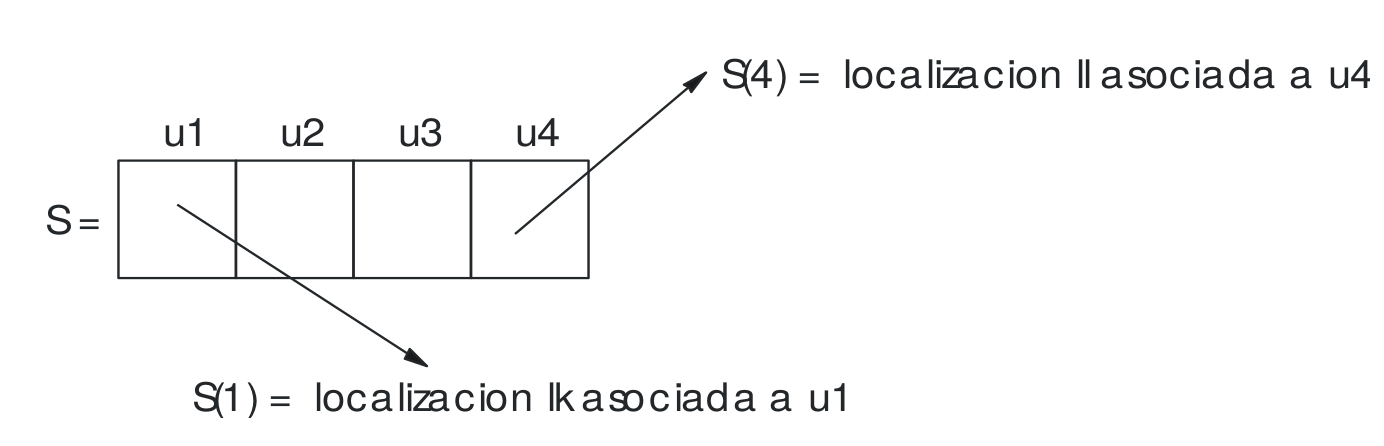
\includegraphics[scale=0.14]{solRep}
   \end{center}
   
   Existe una función \textit{CalcCost} que calcula el coste de dicha solución como:
      $$cost = \sum_{i=1}^{n}\sum_{j=1, j \neq i}^{n} f_{ij}d_{\pi(i)\pi(j)}$$
   donde:
   \begin{itemize}
      \item $\pi$ es la solución al problema.
      
      \item $f_{ij}$ es el flujo que circula entre la unidad $i$ y la $j$.
      
      \item $d_{kl}$ es la distancia existente entre la localización $k$ y la $l$.
   \end{itemize}\vspace*{0.5cm}
   
   Dado que el cálculo del coste de la solución es bastante costoso, $O(n^{2})$, Esta función debe llamarse manualmente al menos una vez para obtener el coste y que este se guarde en la representación de la clase.
   
   
   \newpage
   \section{Algoritmo Greedy}
   Se basa en el cálculo de los potenciales de flujo y distancia definidos como:
   \begin{center}
      $\hat{f}_i = \sum_{j=1}^{n}f_{ij}$ \hspace*{1cm} $\hat{d}_i = \sum_{j=1}^{n}d_{ij}$
   \end{center}
   
   El algoritmo irá seleccionando la unidad $i$ libre con mayor $\hat{f}_i$ y le asignará la localización $j$ libre con menor $\hat{d}_j$. Su implementación en pseudocódigo es la siguiente:  
      \begin{algorithm}
          \# Calcula los potenciales\\
          $dp = fp = vector(n)$\\
          \For{$i=0$ \KwTo $n$}{
             $\hat{f}_i = \hat{d}_i = 0$\\
             \For{$j=0$ \KwTo $n$}{
                $\hat{f}_i = \hat{f}_i + f_{ij}$\\
                $\hat{d}_i = \hat{d}_i + d_{ij}$\\
             }
             $dp_i = \hat{d}_i$\\
             $fp_i = \hat{f}_i$\\
          }\vspace*{0.5cm}
          
          \# Calcula la mejor combinación. $\pi$ es la representación de la solución\\
          $locAssigned = unitAssigned = vector(n)\{0\}$\\
          \For{$i=0$ \KwTo $n$}{
             $best\hat{f} = -\infty$;\hspace*{0.5cm}$best\hat{f}_{index}=0$\\
             $best\hat{d} = \infty$;\hspace*{0.5cm}$best\hat{d}_{index}=0$\\
             \For{$j=0$ \KwTo $n$}{
                $\hat{f}_i = fp_j$;\hspace*{0.5cm}$\hat{d}_i = dp_j$\\
                
                \If{$\hat{f}_i > best\hat{f}$ \textbf{and} $unitAssigned_j \neq 1$}{
                   $best\hat{f} = \hat{f}_i$;\hspace*{0.5cm}$best\hat{f}_{index}=j$\\
                }
                
                \If{$\hat{d}_i < best\hat{d}$  \textbf{and} $locAssigned_j \neq 1$}{
                   $best\hat{d} = \hat{d}_i$;\hspace*{0.5cm}$best\hat{d}_{index}=j$\\
                }
             }
             $\pi(best\hat{f}_{index}) = best\hat{d}_{index}$\\
             $unitAssigned_{best\hat{f}_{index}} = locAssigned_{best\hat{d}_{index}} = 1$\\             
          }
      \end{algorithm}
      
      
      \newpage
      \section{Algoritmo de Búsqueda Local}
      Vamos a utilizar una \textbf{búsqueda local del primer mejor}. Cuando se genera una solución vecina que mejora a la actual, se toma esta como solución y se pasa a la siguiente iteración. Se detiene la búsqueda cuando no se genera ningún vecino mejor que la solución actual. La implementación de dicha idea, que será la función \textit{Solve}, se puede ver como:
      \begin{algorithm}
         $\pi = GenerateInitialSolution()$ \# Será aleatoria\\
         \Do{$\exists \pi'$}{
            $\pi' = GenerateBestNeighbour(\pi)$
            
            \lIf{$\exists \pi'$}{$\pi = \pi'$}
         }
      \end{algorithm}
      
      A fin de minimizar el riesgo de quedarnos en un óptimo local, vamos a partir de una solución aleatoria en vez de partir de una solución greedy. Dicha solución aleatoria se genera de la siguiente manera:
      \begin{algorithm}
         $assigned = vector(n){0}$\\
         \For{$i=0$ \KwTo $n$}{
            \Do{$assigned_r \neq 0$}{
               $r = random() \ mod\ n$\\
             }
             
             $\pi(i) = r$\\
             $assigned_r = 1$\\
         }
      \end{algorithm}
      
      Como se comentó anteriormente, el proceso de cálculo del coste de la solución es de orden cuadrático por lo que realizar dicho calculo con cada vecino es sumamente costoso; En su lugar, vamos a considerar una \textbf{factorización} (con eficiencia $O(n)$) teniendo en cuenta solo los cambios realizados por el movimiento de intercambio para generar el vecino. El incremento del coste de cambiar el elemento en la posición r $r$ por el de $s$ se define como:
      $$
\Delta C(\pi,r,s) = \sum_{k=1, k\neq r,s}^{n}\begin{bmatrix}
f_{rk}(d_{\pi(s)\pi(k)} - d_{\pi(r)\pi(k)}) + f_{sk}(d_{\pi(r)\pi(k)} - d_{\pi(s)\pi(k)}) +\\ 
f_{kr}(d_{\pi(k)\pi(s)} - d_{\pi(k)\pi(r)}) + f_{ks}(d_{\pi(k)\pi(r)} - d_{\pi(k)\pi(s)})
\end{bmatrix} 
      $$
      
      Si $\Delta C(\pi,r,s) < 0$, el resultado de cambiar $r$ por $s$ es favorable, es decir, el costo es menor por lo que tomaremos el vecino resultante de este cambio como solución actual y generamos nuevos vecinos a partir de este.\\
      
      La función que hace uso de esta factorización para explorar los vecinos de una solución se implementaría como:
      \begin{algorithm}
         \SetKwProg{Def}{def}{:}{end}
         \Def{GenerateBestNeighbour($\pi$)}{
            \For{$r=0$ \KwTo $n/2$}{
               \For{$s=r+1$ \KwTo $n$}{                  
                  \If{$\Delta C(\pi,r,s) < 0$}{
                     $\pi' = \pi$\\
                     $t = \pi'(r)$\\
                     $\pi'(r) = \pi'(s)$\\
                     $\pi'(s) = t$\\
                     
                     \textbf{return} $\pi'$
                  }
               }
            }         
         }
      \end{algorithm}
      
      Como vemos, podemos reducir considerablemente el numero de iteraciones totales iterando en $r$ en el primer bucle hasta $n/2$ y en el segundo desde $r+1$ hasta $n$, ya que así podemos evitar comparar dos veces el mismo movimiento. Es lo mismo cambiar $r$ por $s$ que $s$ por $r$.
     
      
      \newpage
      \subsection*{Búsqueda Local con \textit{Don't Look Bits}}
      Como estamos utilizando una \textbf{búsqueda local del primer mejor}, podemos definir una lista de candidatos a la que llamamos \textbf{\textit{Don't Look Bits}} que reducirá significativamente el tiempo de ejecución.\\
      
      Se trata de un un vector de bits inicialmente a 0, esto nos indica que todos los movimientos pueden ser considerados. Si tras probar todos los movimientos asociados un bit no hemos encontrado ninguna mejora, cambiaremos el valor de dicho bit a 1, indicando que esta unidad no debe ser tenida en cuenta hasta que dicha unidad asociada a ese bit se vea implicada en un movimiento que mejora la solución actual, en cuyo caso el bit será nuevamente 0.\\
      
      Podemos ejemplificar este algoritmo con el siguiente pseudocódigo:
      \begin{algorithm}
         $dlbMask = vector(n)\{0\}$ \# Don't look bits\\
         \SetKwProg{Def}{def}{:}{end}
         \Def{GenerateBestNeighbour($\pi$)}{
            \For{$r=0$ \KwTo $n$}{
               \lIf{$dlbMask_r \neq 0$}{\textbf{continue}}
               \For{$s=0$ \KwTo $n$}{                  
                  \If{$\Delta C(\pi,r,s) < 0$}{
                     $\pi' = \pi$\\
                     $t = \pi'(r)$\\
                     $\pi'(r) = \pi'(s)$\\
                     $\pi'(s) = t$\\
                     
                     $dlbMask_r = dlbMask_s = 0$\\
                     \textbf{return} $\pi'$
                  }
               }
               $dlbMask_r = 1$
            }         
         }
      \end{algorithm}
      
      
      \newpage
      \section{Procedimiento considerado para desarrollar la práctica}
      Esta práctica ha sido desarrollada en \textbf{C++} como una librería de metaheurísticas. La estructura del proyecto es la siguiente:\\
      
      \dirtree{%
         .1 /Software.
         .2 bin/         \DTcomment{Archivos ejecutables}.
         .3 practica1   \DTcomment{Ejecutable principal de la práctica}.
         .2 build/       \DTcomment{Directorio para compilación con CMake}.
         .2 doc/         \DTcomment{Otra documentación y código LaTeX de este documento}.
         .2 include/     \DTcomment{Cabeceras}.
         .2 instancias/  \DTcomment{Instancias de problemas sobre QAP}.
         .3 *.dat   \DTcomment{Definición de un problema}.
         .3 *.sln   \DTcomment{Solución a un problema}.
         .2 src/         \DTcomment{Código fuente}.
         .2 CMakeLists.txt   \DTcomment{Instrucciones de compilación para CMake}.
         .2 readme.txt       \DTcomment{Instrucciones de uso}.
      }\vspace*{0.5cm}
      
      Para compilar este proyecto necesitamos las herramientas \textit{g++} y \textit{CMake}. Para instalarlas en un sistema \textbf{Ubuntu} o derivado, ejecutamos:
      
      \begin{lstlisting}[language=bash]
      sudo apt-get install g++ cmake 
      \end{lstlisting}
      
      Podemos compilar el proyecto con dos niveles de optimización:
      \begin{itemize}
         \item \textbf{Debug}: Sin optimización y con símbolos de depuración. Ejecutar CMake con opción \textit{-D CMAKE\_BUILD\_TYPE=Debug}
         
         \item \textbf{Release}: Máxima optimización en la compilación. Por defecto.
      \end{itemize}
      
      Se compila con las siguientes instrucciones:
      
      \begin{lstlisting}[language=bash]
   cd build/
   # Para debug: cmake -D CMAKE_BUILD_TYPE=Debug ..
   cmake ..  
   make clean
   make
   cd ..
      \end{lstlisting}
      
      \newpage
      La sintaxis de ejecución es la siguiente\footnote{Todo en la misma línea. El parámetro semilla es opcional, por defecto $semilla = 7$}:
      \begin{lstlisting}[language=bash]
./bin/practica1 instancias/<problema>.dat 
                <ruta_escribir_solucion> 
                <semilla>
      \end{lstlisting}
      
      Por ejemplo:
      \begin{lstlisting}[language=bash]
./bin/practica1 instancias/chr22a.dat prueba.sln 12
      \end{lstlisting}
      
      La salida del programa tiene la siguiente estructura:
      \begin{center}
      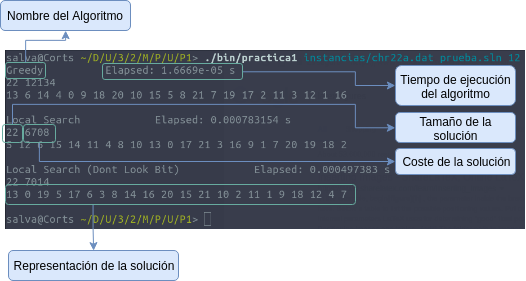
\includegraphics[scale=0.7]{execOutDiagram}
      \end{center}
      
      
      \newpage
      \section{Experimentos y análisis de resultados}
      Con el fin de comparar los algoritmos implementados con los ya existentes, vamos a calcular para cada algoritmo los siguientes parámetros:
      \begin{itemize}
         \item \textbf{\textit{Desv}}: Media de las desviaciones en porcentaje, del valor obtenido por cada método en cada instancia respecto al mejor valor conocido para ese caso.
         $$ \frac{1}{\left | casos \right |}\sum_{i=1}^{casos}100\frac{valoralgoritmo_i - mejorValor_i}{mejorValor_i} $$
         Obtendremos los mejores valores conocidos de \textit{QAPLIB}\footnote{http://anjos.mgi.polymtl.ca/qaplib//inst.html}
         
         \item \textbf{\textit{Tiempo}}: se calcula como la media del tiempo de ejecución empleado por el
algoritmo para resolver cada caso del problema.
      \end{itemize}
      
      Cuanto menor es el valor de Desv para un algoritmo, mejor calidad tiene dicho algoritmo. Por otro lado, si dos métodos obtienen soluciones de la misma calidad (tienen valores de Desv similares), uno será mejor que el otro si emplea menos tiempo en media.\\
      
\emph{\textbf{Parámetros del experimento:} 
   \begin{itemize}
      \item El valor de la semilla para este experimento es 7.
      \item Se compilara con parámetro \textbf{debug} a fin de contrastar aún mas los resultados del tiempo.
   \end{itemize}
}      

      
      \newpage
      \subsection*{Resultados Greedy}
\begin{table}[H]
\centering
\caption{goo.gl/yr6uN9}
\label{my-label}
\begin{tabular}{|l|l|l|l|l|l|l|}
\hline
\multicolumn{7}{|c|}{\textbf{Algoritmo Greedy}}                                                                                                                                                \\ \hline
\textbf{Caso}    & \multicolumn{1}{c|}{\textbf{Desv}} & \multicolumn{1}{c|}{\textbf{Tiempo}} &  & \textbf{Caso}    & \multicolumn{1}{c|}{\textbf{Desv}} & \multicolumn{1}{c|}{\textbf{Tiempo}} \\ \cline{1-3} \cline{5-7} 
\textbf{Chr22a}  & 97,11                              & 0,000126925                          &  & \textbf{Sko100a} & 13,36                              & 0,000630563                          \\ \cline{1-3} \cline{5-7} 
\textbf{Chr22b}  & 134,48                             & 0,000125567                          &  & \textbf{Sko100f} & 13,77                              & 0,00230857                           \\ \cline{1-3} \cline{5-7} 
\textbf{Chr25a}  & 448,47                             & 0,000175691                          &  & \textbf{Tai100a} & 13,80                              & 0,000616869                          \\ \cline{1-3} \cline{5-7} 
\textbf{Esc128}  & 140,63                             & 0,00117301                           &  & \textbf{Tai100b} & 32,79                              & 0,000626035                          \\ \cline{1-3} \cline{5-7} 
\textbf{Had20}   & 7,71                               & 0,000102693                          &  & \textbf{Tai150b} & 24,97                              & 0,00136394                           \\ \cline{1-3} \cline{5-7} 
\textbf{Lipa60b} & 27,59                              & 0,000289296                          &  & \textbf{Tai256c} & 120,48                             & 0,00340613                           \\ \cline{1-3} \cline{5-7} 
\textbf{Lipa80b} & 28,58                              & 0,000382927                          &  & \textbf{Tho40}   & 29,96                              & 0,000384573                          \\ \cline{1-3} \cline{5-7} 
\textbf{Nug28}   & 22,88                              & 0,00020704                           &  & \textbf{Tho150}  & 16,98                              & 0,00204635                           \\ \cline{1-3} \cline{5-7} 
\textbf{Sko81}   & 15,50                              & 0,0013694                            &  & \textbf{Wil50}   & 11,68                              & 0,00017995                           \\ \cline{1-3} \cline{5-7} 
\textbf{Sko90}   & 13,61                              & 0,00162198                           &  & \textbf{Wil100}  & 7,33                               & 0,000619954                          \\ \cline{1-3} \cline{5-7} 
\end{tabular}
\end{table}

      Como podríamos esperar, el algoritmo greedy es muy rápido, aunque las soluciones obtenidas distan bastante de la mejor conocida. Podríamos discutir su utilidad desde un punto de vista práctico; ¿En qué escenarios puede sernos útil una búsqueda greedy?
      
      \begin{enumerate}
         \item Si ofrecemos un servicio donde la optimalidad de la solución a un problema es lo de menos y tenemos que responder muchas solicitudes con pocos recursos de manera muy rápida.
         
         \item Como algoritmo auxiliar de cara a obtener una solución inicial para posteriormente tratar de mejorarla mediante el uso de algoritmos mas complejos. No obstante, esto no siempre es buena idea pues corremos el riesgo de caer en óptimos locales. Hay que usarlos con algoritmos que sean capaces de esquivar con relativa facilidad óptimos locales.         
      \end{enumerate}

      
      \newpage
      \subsection*{Resultados Búsqueda Local}
\begin{table}[H]
\centering
\caption{goo.gl/SJJh1a}
\label{my-label}
\begin{tabular}{|l|l|l|l|l|l|l|}
\hline
\multicolumn{7}{|c|}{\textbf{Algoritmo Búsqueda Local}}                                                                                                                                    \\ \hline
\textbf{Caso}    & \multicolumn{1}{c|}{\textbf{Desv}} & \multicolumn{1}{c|}{\textbf{Tiempo}} &  & \textbf{Caso}    & \multicolumn{1}{c|}{\textbf{Desv}} & \multicolumn{1}{c|}{\textbf{Tiempo}} \\ \cline{1-3} \cline{5-7} 
\textbf{Chr22a}  & 17,41                              & 0,00255601                           &  & \textbf{Sko100a} & 2,53                               & 1,54504                              \\ \cline{1-3} \cline{5-7} 
\textbf{Chr22b}  & 15,63                              & 0,00382979                           &  & \textbf{Sko100f} & 2,21                               & 2,05617                              \\ \cline{1-3} \cline{5-7} 
\textbf{Chr25a}  & 75,40                              & 0,00940898                           &  & \textbf{Tai100a} & 3,35                               & 0,806562                             \\ \cline{1-3} \cline{5-7} 
\textbf{Esc128}  & 18,75                              & 0,360157                             &  & \textbf{Tai100b} & 4,94                               & 3,26802                              \\ \cline{1-3} \cline{5-7} 
\textbf{Had20}   & 1,44                               & 0,0058809                            &  & \textbf{Tai150b} & 3,50                               & 24,8278                              \\ \cline{1-3} \cline{5-7} 
\textbf{Lipa60b} & 19,79                              & 0,114542                             &  & \textbf{Tai256c} & 1,26                               & 5,15624                              \\ \cline{1-3} \cline{5-7} 
\textbf{Lipa80b} & 22,30                              & 0,291904                             &  & \textbf{Tho40}   & 5,34                               & 0,0626425                            \\ \cline{1-3} \cline{5-7} 
\textbf{Nug28}   & 8,94                               & 0,0114589                            &  & \textbf{Tho150}  & 2,78                               & 13,1679                              \\ \cline{1-3} \cline{5-7} 
\textbf{Sko81}   & 2,70                               & 0,540895                             &  & \textbf{Wil50}   & 1,96                               & 0,10151                              \\ \cline{1-3} \cline{5-7} 
\textbf{Sko90}   & 1,86                               & 1,46495                              &  & \textbf{Wil100}  & 1,07                               & 2,19904                              \\ \cline{1-3} \cline{5-7} 
\end{tabular}
\end{table}

      Aunque no se obtienen soluciones óptimas, estas están muy cerca de serlo. Podemos apreciar que este algoritmo trabaja muy bien con problemas relativamente pequeños pero dado que, a diferencia del greedy, el tiempo crece significativamente en función del tamaño del problema, utilizarlo como algoritmo de propósito general para solucionar problemas no es lo idóneo.\\
      
      Sin embargo, en combinación con otros algoritmos como los Genéticos podemos obtener resultados aún mejores y en un tiempo mas aceptable dado que restringimos el espacio de búsqueda para este algoritmo.


      
      \newpage
      \subsection*{Resultados Búsqueda Local con \textit{Don't Look Bits}}
\begin{table}[H]
\caption{goo.gl/9frEmN}
\centering
\label{my-label}
\begin{tabular}{|l|l|l|l|l|l|l|}
\hline
\multicolumn{7}{|c|}{\textbf{Algoritmo Búsqueda Local DLB}}                                                                                                                                    \\ \hline
\textbf{Caso}    & \multicolumn{1}{c|}{\textbf{Desv}} & \multicolumn{1}{c|}{\textbf{Tiempo}} &  & \textbf{Caso}    & \multicolumn{1}{c|}{\textbf{Desv}} & \multicolumn{1}{c|}{\textbf{Tiempo}} \\ \cline{1-3} \cline{5-7} 
\textbf{Chr22a}  & 18.23                              & 0,0020404                            &  & \textbf{Sko100a} & 2.78                               & 0,229239                             \\ \cline{1-3} \cline{5-7} 
\textbf{Chr22b}  & 9.07                               & 0,0059782                            &  & \textbf{Sko100f} & 2.5                                & 0,226626                             \\ \cline{1-3} \cline{5-7} 
\textbf{Chr25a}  & 43.52                              & 0,00274717                           &  & \textbf{Tai100a} & 4.12                               & 0,164417                             \\ \cline{1-3} \cline{5-7} 
\textbf{Esc128}  & 12.5                               & 0,193508                             &  & \textbf{Tai100b} & 4.89                               & 0,418418                             \\ \cline{1-3} \cline{5-7} 
\textbf{Had20}   & 2.11                               & 0,00561109                           &  & \textbf{Tai150b} & 2.59                               & 1,5031                               \\ \cline{1-3} \cline{5-7} 
\textbf{Lipa60b} & 20.23                              & 0,0302634                            &  & \textbf{Tai256c} & 0.79                               & 1,84737                              \\ \cline{1-3} \cline{5-7} 
\textbf{Lipa80b} & 22.08                              & 0,0758918                            &  & \textbf{Tho40}   & 6.52                               & 0,0116882                            \\ \cline{1-3} \cline{5-7} 
\textbf{Nug28}   & 3.45                               & 0,0058682                            &  & \textbf{Tho150}  & 2.18                               & 1,14028                              \\ \cline{1-3} \cline{5-7} 
\textbf{Sko81}   & 2.1                                & 0,141866                             &  & \textbf{Wil50}   & 1.7                                & 0,0221609                            \\ \cline{1-3} \cline{5-7} 
\textbf{Sko90}   & 2.67                               & 0,246332                             &  & \textbf{Wil100}  & 1.26                               & 0,252535                             \\ \cline{1-3} \cline{5-7} 
\end{tabular}
\end{table}

      Podemos observar que la técnica de \textit{Don't look bits} mejora significativamente los tiempos de ejecución de la versión basica de la búsqueda local. 
      
      
      
      
      
      \newpage
      \subsection*{Comparación de los resultados. Conclusiones.}
\begin{table}[H]
\centering
\label{my-label}
\begin{tabular}{|l|l|l|}
\hline
\multicolumn{1}{|c|}{\textbf{Algoritmo}} & \textbf{Desv} & \multicolumn{1}{c|}{\textbf{Tiempo}} \\ \hline
\textbf{Greedy}                          & 61,08         & 0,00088787315                        \\ \hline
\textbf{BL}                              & 10,66         & 2,80                                 \\ \hline
\textbf{BL. Don't Look Bits}             & 8.26          & 0,33                                 \\ \hline
\end{tabular}
\end{table}
      
      Como podemos ver, el tiempo de ejecución del algoritmo greedy es varias magnitudes menor que los tiempos de los otros dos algoritmos. Sin embargo, la poca calidad de sus soluciones hace que, por si sola, no sea una herramienta idónea de cara a resolver problemas.\\
      
      Tanto la Búsqueda Local básica como su variante con \textit{Dont't look bits} nos ofrecen resultados mucho mas óptimos que el greedy. \\
      
      Como la desviación de BL y BL con DLB es similar, debemos fijarnos en el tiempo medio de ejecución. La variante \textit{DLB} es 8.5\footnote{$2.80/0.33 = 8.\overline{48}$} veces más rápida que la original. Aunque la variante \textit{Don't Look Bits} ofrece resultados ligeramente mejores, esto no debe ser tomado como referencia, pues la naturaleza aleatoria de cara a generar la solución de partida hace que no podamos asegurar que uno encuentra siempre una solución mejor que la otra.\\
      
      Cabe destacar que el experimento ha sido compilado sin optimización (\textbf{\textit{Debug}}). La realidad es que con un nivel máximo de optimización (\textbf{\textit{Release}}), aún en problemas de mayor tamaño y complejidad como \textbf{\textit{Tai150b}} obtenemos unos tiempos mucho menores que hace que utilizar un greedy en producción sea aun menos viable.\\
      
      Un ejemplo ilustrativo de la diferencia de tiempos en función del nivel de optimización:
      
\begin{table}[H]
\centering
\label{my-label}
\begin{tabular}{l|c|c|}
\cline{2-3}
\multicolumn{1}{c|}{{\textit{Tai150b}}} & \multicolumn{2}{c|}{\textbf{Nivel de Optimización}} \\ \hline
\multicolumn{1}{|c|}{\textbf{Algoritmo}}    & \textbf{Debug}          & \textbf{Release}          \\ \hline
\multicolumn{1}{|l|}{\textbf{BL}}           & 24.174                  & 1.55584                   \\ \hline
\multicolumn{1}{|l|}{\textbf{BL DLB}}       & 1.54554                 & 0.105939                  \\ \hline
\end{tabular}
\end{table}
   
\printindex
\end{document}
